% Options for packages loaded elsewhere
\PassOptionsToPackage{unicode}{hyperref}
\PassOptionsToPackage{hyphens}{url}
\PassOptionsToPackage{dvipsnames,svgnames,x11names}{xcolor}
%
\documentclass[
]{agujournal2019}

\usepackage{amsmath,amssymb}
\usepackage{iftex}
\ifPDFTeX
  \usepackage[T1]{fontenc}
  \usepackage[utf8]{inputenc}
  \usepackage{textcomp} % provide euro and other symbols
\else % if luatex or xetex
  \usepackage{unicode-math}
  \defaultfontfeatures{Scale=MatchLowercase}
  \defaultfontfeatures[\rmfamily]{Ligatures=TeX,Scale=1}
\fi
\usepackage{lmodern}
\ifPDFTeX\else  
    % xetex/luatex font selection
\fi
% Use upquote if available, for straight quotes in verbatim environments
\IfFileExists{upquote.sty}{\usepackage{upquote}}{}
\IfFileExists{microtype.sty}{% use microtype if available
  \usepackage[]{microtype}
  \UseMicrotypeSet[protrusion]{basicmath} % disable protrusion for tt fonts
}{}
\makeatletter
\@ifundefined{KOMAClassName}{% if non-KOMA class
  \IfFileExists{parskip.sty}{%
    \usepackage{parskip}
  }{% else
    \setlength{\parindent}{0pt}
    \setlength{\parskip}{6pt plus 2pt minus 1pt}}
}{% if KOMA class
  \KOMAoptions{parskip=half}}
\makeatother
\usepackage{xcolor}
\setlength{\emergencystretch}{3em} % prevent overfull lines
\setcounter{secnumdepth}{5}
% Make \paragraph and \subparagraph free-standing
\ifx\paragraph\undefined\else
  \let\oldparagraph\paragraph
  \renewcommand{\paragraph}[1]{\oldparagraph{#1}\mbox{}}
\fi
\ifx\subparagraph\undefined\else
  \let\oldsubparagraph\subparagraph
  \renewcommand{\subparagraph}[1]{\oldsubparagraph{#1}\mbox{}}
\fi


\providecommand{\tightlist}{%
  \setlength{\itemsep}{0pt}\setlength{\parskip}{0pt}}\usepackage{longtable,booktabs,array}
\usepackage{calc} % for calculating minipage widths
% Correct order of tables after \paragraph or \subparagraph
\usepackage{etoolbox}
\makeatletter
\patchcmd\longtable{\par}{\if@noskipsec\mbox{}\fi\par}{}{}
\makeatother
% Allow footnotes in longtable head/foot
\IfFileExists{footnotehyper.sty}{\usepackage{footnotehyper}}{\usepackage{footnote}}
\makesavenoteenv{longtable}
\usepackage{graphicx}
\makeatletter
\def\maxwidth{\ifdim\Gin@nat@width>\linewidth\linewidth\else\Gin@nat@width\fi}
\def\maxheight{\ifdim\Gin@nat@height>\textheight\textheight\else\Gin@nat@height\fi}
\makeatother
% Scale images if necessary, so that they will not overflow the page
% margins by default, and it is still possible to overwrite the defaults
% using explicit options in \includegraphics[width, height, ...]{}
\setkeys{Gin}{width=\maxwidth,height=\maxheight,keepaspectratio}
% Set default figure placement to htbp
\makeatletter
\def\fps@figure{htbp}
\makeatother
% definitions for citeproc citations
\NewDocumentCommand\citeproctext{}{}
\NewDocumentCommand\citeproc{mm}{%
  \begingroup\def\citeproctext{#2}\cite{#1}\endgroup}
\makeatletter
 % allow citations to break across lines
 \let\@cite@ofmt\@firstofone
 % avoid brackets around text for \cite:
 \def\@biblabel#1{}
 \def\@cite#1#2{{#1\if@tempswa , #2\fi}}
\makeatother
\newlength{\cslhangindent}
\setlength{\cslhangindent}{1.5em}
\newlength{\csllabelwidth}
\setlength{\csllabelwidth}{3em}
\newenvironment{CSLReferences}[2] % #1 hanging-indent, #2 entry-spacing
 {\begin{list}{}{%
  \setlength{\itemindent}{0pt}
  \setlength{\leftmargin}{0pt}
  \setlength{\parsep}{0pt}
  % turn on hanging indent if param 1 is 1
  \ifodd #1
   \setlength{\leftmargin}{\cslhangindent}
   \setlength{\itemindent}{-1\cslhangindent}
  \fi
  % set entry spacing
  \setlength{\itemsep}{#2\baselineskip}}}
 {\end{list}}
\usepackage{calc}
\newcommand{\CSLBlock}[1]{\hfill\break\parbox[t]{\linewidth}{\strut\ignorespaces#1\strut}}
\newcommand{\CSLLeftMargin}[1]{\parbox[t]{\csllabelwidth}{\strut#1\strut}}
\newcommand{\CSLRightInline}[1]{\parbox[t]{\linewidth - \csllabelwidth}{\strut#1\strut}}
\newcommand{\CSLIndent}[1]{\hspace{\cslhangindent}#1}

\usepackage{url} %this package should fix any errors with URLs in refs.
\usepackage{lineno}
\usepackage[inline]{trackchanges} %for better track changes. finalnew option will compile document with changes incorporated.
\usepackage{soul}
\linenumbers
\makeatletter
\@ifpackageloaded{caption}{}{\usepackage{caption}}
\AtBeginDocument{%
\ifdefined\contentsname
  \renewcommand*\contentsname{Table of contents}
\else
  \newcommand\contentsname{Table of contents}
\fi
\ifdefined\listfigurename
  \renewcommand*\listfigurename{List of Figures}
\else
  \newcommand\listfigurename{List of Figures}
\fi
\ifdefined\listtablename
  \renewcommand*\listtablename{List of Tables}
\else
  \newcommand\listtablename{List of Tables}
\fi
\ifdefined\figurename
  \renewcommand*\figurename{Figure}
\else
  \newcommand\figurename{Figure}
\fi
\ifdefined\tablename
  \renewcommand*\tablename{Table}
\else
  \newcommand\tablename{Table}
\fi
}
\@ifpackageloaded{float}{}{\usepackage{float}}
\floatstyle{ruled}
\@ifundefined{c@chapter}{\newfloat{codelisting}{h}{lop}}{\newfloat{codelisting}{h}{lop}[chapter]}
\floatname{codelisting}{Listing}
\newcommand*\listoflistings{\listof{codelisting}{List of Listings}}
\makeatother
\makeatletter
\makeatother
\makeatletter
\@ifpackageloaded{caption}{}{\usepackage{caption}}
\@ifpackageloaded{subcaption}{}{\usepackage{subcaption}}
\makeatother
\ifLuaTeX
  \usepackage{selnolig}  % disable illegal ligatures
\fi
\usepackage{bookmark}

\IfFileExists{xurl.sty}{\usepackage{xurl}}{} % add URL line breaks if available
\urlstyle{same} % disable monospaced font for URLs
\hypersetup{
  pdftitle={Near Infra-Red Spectroscopy Predicts Crude Protein in Hemp Grain},
  pdfauthor={Ryan Crawford; Lawrence B. Smart; Virginia Moore},
  pdfkeywords={La Palma, Earthquakes},
  colorlinks=true,
  linkcolor={blue},
  filecolor={Maroon},
  citecolor={Blue},
  urlcolor={Blue},
  pdfcreator={LaTeX via pandoc}}

\journalname{Earth and Space Science}

\draftfalse

\begin{document}
\title{Near Infra-Red Spectroscopy Predicts Crude Protein in Hemp Grain}

\authors{Ryan Crawford\affil{1}, Lawrence B. Smart\affil{2,3}, Virginia
Moore\affil{4}}
\affiliation{1}{Cornell University, Ithaca, NY, }\affiliation{2}{Cornell
AgriTech, Geneva, NY, }\affiliation{3}{Curvenote, }\affiliation{4}{Cornell
University, Ithaca, NY, }
\correspondingauthor{Ryan Crawford}{rvc3@cornell.edu}


\begin{abstract}
Lorem ipsum dolor sit amet, consectetur adipiscing elit, sed do eiusmod
tempor incididunt ut labore et dolore magna aliqua. Ut enim ad minim
veniam, quis nostrud exercitation ullamco laboris nisi ut aliquip ex ea
commodo consequat. Duis aute irure dolor in reprehenderit in voluptate
velit esse cillum dolore eu fugiat nulla pariatur. Excepteur sint
occaecat cupidatat non proident, sunt in culpa qui officia deserunt
mollit anim id est laborum.
\end{abstract}

\section*{Plain Language Summary}
Earthquake data for the island of La Palma from the September 2021
eruption is found \ldots{}



\section{ABSTRACT}\label{abstract}

\section{INTRODUCTION}\label{introduction}

Hemp (Cannabis sativa L.) is an annual crop with potential uses as a
source of food or feed from grain, and bast fiber or hurd from the
stalk. Hemp cultivars are commonly grown for one or both purposes.

Percentage crude protein (CP) of grain is an important consideration for
researchers, producers, and consumers.

Protein is important because of its nutrition

Near-infrared spectroscopy (NIRS) technology is rapid, non-destructive,
and cheap. Within the context of plant breeding, a sample of undamaged
grain may subsequently be planted. NIRS technology has been used since
the 1970's to assess oil seeds Williams (1975)

A calibration set typically consists of samples from many environments
encompassing the range of expected values from the analyte (Chadalavada
et al., 2022). For this study, a benchtop NIR spectrometer was used to
develop a model to predict crude protein content based on a data set
representing multiple years, locations, and cultivars.

\section{MATERIALS AND METHODS}\label{materials-and-methods}

\textsubscript{Source:
\href{https://rvcrawford.github.io/glowing-system/index.qmd.html}{Article
Notebook}}

\subsection{Hemp Grain Sample
Background}\label{hemp-grain-sample-background}

Spectral data were obtained from whole (unground) hemp grain samples,
harvested at maturity, collected from 2017 - 2021 from 18 cultivar
trials in New York (NY) (149 samples). Grain samples were obtained by
hand sampling or mechanical harvest and were cleaned of chaff and dried
at 30 C for six days in a forced-air dryer. In total, 39 cultivars were
represented in the data set. Cultivars were grain or dual-purpose types
and included both commercially available and experimental material.

All cultivar trials were planted in randomized complete block design
with each cultivar replicated four times. The 2017 data were comprised
of samples from the same thirteen cultivars sampled from six NY
locations. For those trials, grain was harvested from each plot
individually and aggregated by cultivar. Four subsamples were drawn from
each aggregated sample and scanned separately. These spectra were
averaged at each 2 nm increment. All remaining samples from 2018 - 2021
were collected on a per-plot basis. All possible cultivars and possible
locations were represented in 2017, but only a selected subset of
cultivars and locations were represented in 2018-2021.

\subsection{Spectral Data Collection}\label{spectral-data-collection}

A benchtop NIR spectrometer (FOSS/ NIR FOSS/ NIR Systems model 5000) was
used to obtain the spectra (FOSS North America, Eden Prairie, MN, USA).
Spectra were collected every 2 nm from 1100-2498 nm and the logarithm of
reciprocal reflectance was recorded.

WINISI software version 1.02A (Infrasoft International, Port Matilda,
PA, USA) was used to average the spectra in 2017, as well as to select
samples for crude protein laboratory assay from 2018-2021. Samples were
selected for assay according to their spectral distance from their
nearest neighbor within the calibration data set with a cutoff of a
distance of 0.6 H, where H is approximately equal to the squared
Mahalanobis distance divided by the number of principal components used
in the calculation (\textbf{garrido-varo2019?}). For selection, spectra
were preprocessed using SNV-detrend with settings 1,4,4,1 for the
derivative, gap, smooth, and smooth 2 settings respectively.

\subsection{Software used:}\label{software-used}

Additional analysis was performed

\subsection{Preprocessing}\label{preprocessing}

Multiplicative scatter correction (MSC)

standard normal variate (SNV) transformation

The calibration set consisted of

The validation set consisted of

Laboratory assays were performed by Dairy One Forage Laboratory (Ithaca,
NY). For those assays, 1mm ground samples were analyzed by combustion
using a CN628 or CN928 Carbon/Nitrogen Determinator.

Prior to In 2017, an in

\section{RESULTS AND DISCUSSION}\label{results-and-discussion}

\section{ACKNOWLEDGMENTS}\label{acknowledgments}

\section{SUPPLEMENTAL MATERIAL}\label{supplemental-material}

\section{OPTIONAL SECTIONS}\label{optional-sections}

\section{REFERENCES}\label{references}

\section{FIGURES AND TABLES}\label{figures-and-tables}

\textsubscript{Source:
\href{https://rvcrawford.github.io/glowing-system/index.qmd.html}{Article
Notebook}}

\phantomsection\label{cell-fig-timeline}
\begin{figure}[H]

\centering{

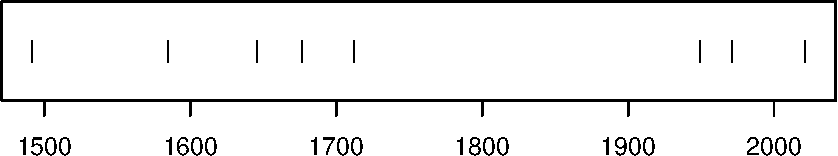
\includegraphics{index_files/figure-pdf/fig-timeline-1.pdf}

}

\caption{\label{fig-timeline}Timeline of recent earthquakes on La Palma}

\end{figure}%

\textsubscript{Source:
\href{https://rvcrawford.github.io/glowing-system/index.qmd.html}{Article
Notebook}}

\textsubscript{Source:
\href{https://rvcrawford.github.io/glowing-system/index.qmd.html}{Article
Notebook}}

Based on data up to and including 1971, eruptions on La Palma happen
every 79.8 years on average.

Studies of the magma systems feeding the volcano, such as Marrero et al.
(2019), have proposed that there are two main magma reservoirs feeding
the Cumbre Vieja volcano; one in the mantle (30-40km depth) which
charges and in turn feeds a shallower crustal reservoir (10-20km depth).

Eight eruptions have been recorded since the late 1400s
(Figure~\ref{fig-timeline}).

Data and methods are discussed in Section~\ref{sec-data-methods}.

Let \(x\) denote the number of eruptions in a year. Then, \(x\) can be
modeled by a Poisson distribution

\begin{equation}\phantomsection\label{eq-poisson}{
p(x) = \frac{e^{-\lambda} \lambda^{x}}{x !}
}\end{equation}

where \(\lambda\) is the rate of eruptions per year. Using
Equation~\ref{eq-poisson}, the probability of an eruption in the next
\(t\) years can be calculated.

\begin{longtable}[]{@{}ll@{}}
\caption{Recent historic eruptions on La
Palma}\label{tbl-history}\tabularnewline
\toprule\noalign{}
Name & Year \\
\midrule\noalign{}
\endfirsthead
\toprule\noalign{}
Name & Year \\
\midrule\noalign{}
\endhead
\bottomrule\noalign{}
\endlastfoot
Current & 2021 \\
Teneguía & 1971 \\
Nambroque & 1949 \\
El Charco & 1712 \\
Volcán San Antonio & 1677 \\
Volcán San Martin & 1646 \\
Tajuya near El Paso & 1585 \\
Montaña Quemada & 1492 \\
\end{longtable}

Table~\ref{tbl-history} summarises the eruptions recorded since the
colonization of the islands by Europeans in the late 1400s.

\begin{figure}

\centering{

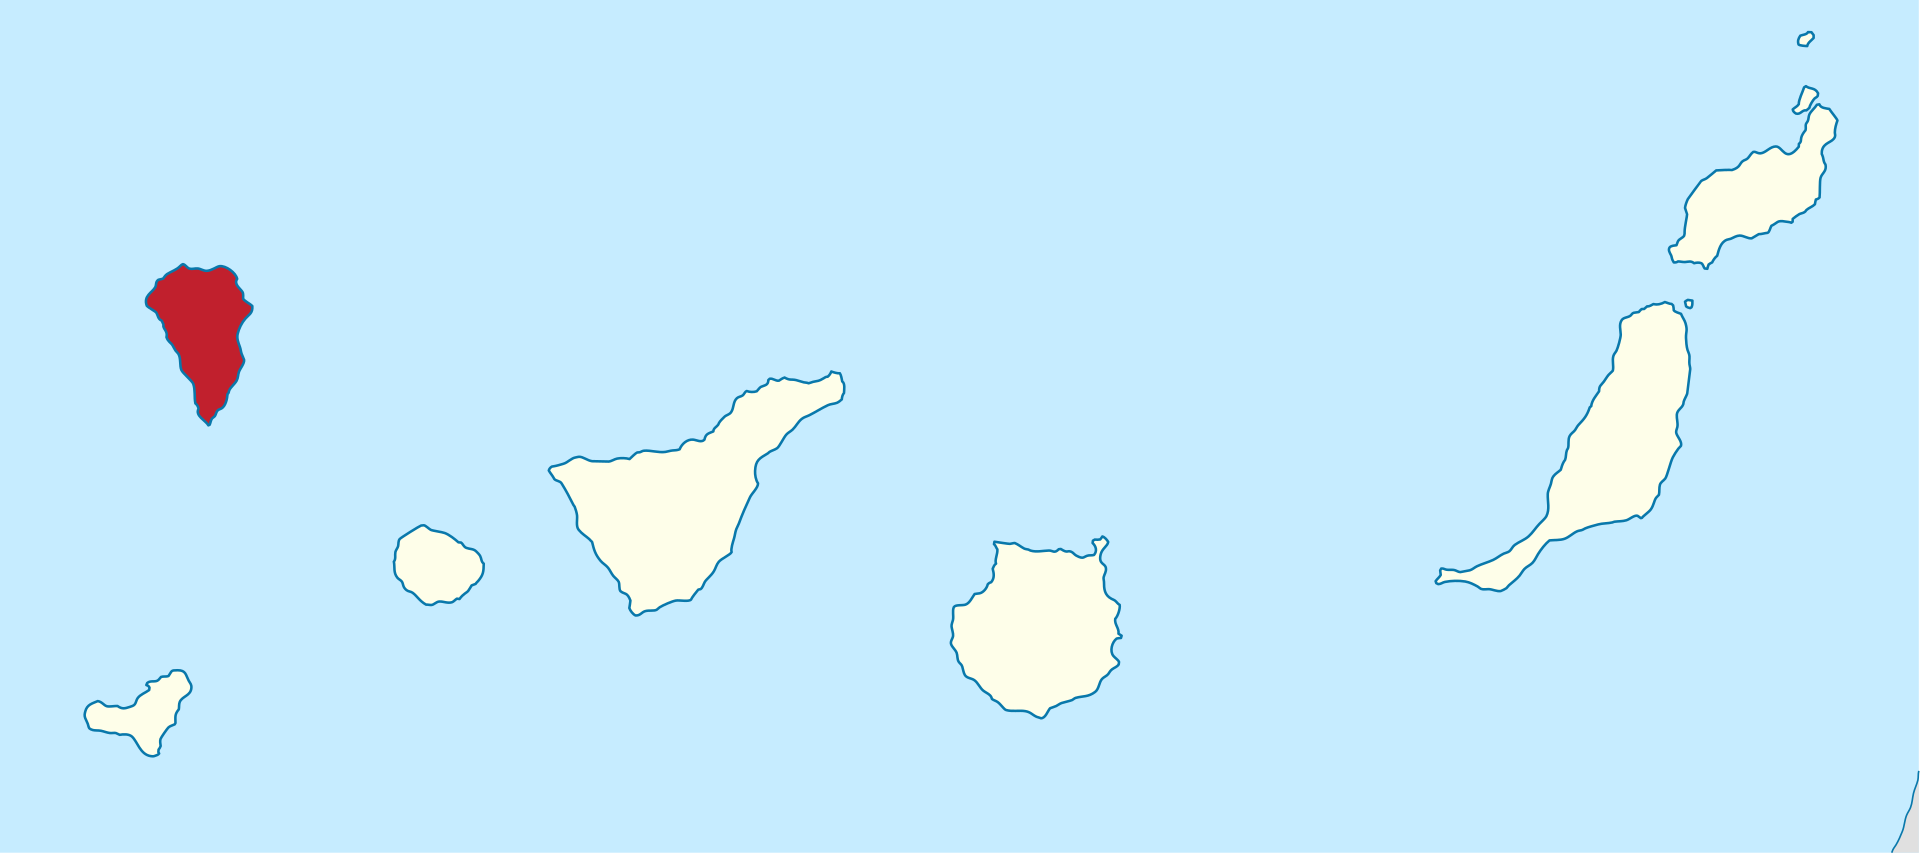
\includegraphics{images/la-palma-map.png}

}

\caption{\label{fig-map}Map of La Palma}

\end{figure}%

La Palma is one of the west most islands in the Volcanic Archipelago of
the Canary Islands (Figure~\ref{fig-map}).

\begin{figure}[H]

\centering{

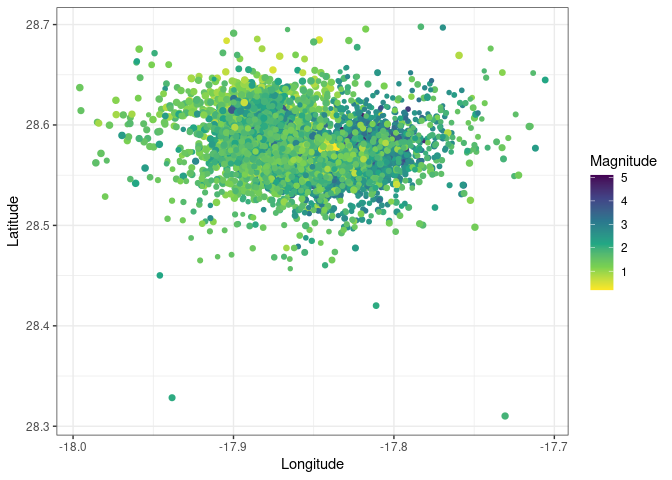
\includegraphics{index_files/figure-latex/notebooks-explore-earthquakes-fig-spatial-plot-output-1.png}

}

\caption{\label{fig-spatial-plot}Locations of earthquakes on La Palma
since 2017}

\end{figure}%

\textsubscript{Source:
\href{https://rvcrawford.github.io/glowing-system/notebooks/explore-earthquakes-preview.html\#cell-fig-spatial-plot}{Explore
Earthquakes}}

Figure~\ref{fig-spatial-plot} shows the location of recent Earthquakes
on La Palma.

\section{Data \& Methods}\label{sec-data-methods}

\section{Conclusion}\label{conclusion}

\section*{References}\label{references-1}
\addcontentsline{toc}{section}{References}

\phantomsection\label{refs}
\begin{CSLReferences}{1}{0}
\vspace{1em}

\bibitem[\citeproctext]{ref-chadalavada_nir_2022}
Chadalavada, K., Anbazhagan, K., Ndour, A., Choudhary, S., Palmer, W.,
Flynn, J. R., Mallayee, S., Pothu, S., Prasad, K. V. S. V.,
Varijakshapanikar, P., Jones, C. S., \& Kholová, J. (2022). {NIR}
{Instruments} and {Prediction} {Methods} for {Rapid} {Access} to {Grain}
{Protein} {Content} in {Multiple} {Cereals}. \emph{Sensors (Basel,
Switzerland)}, \emph{22}(10). \url{https://doi.org/10.3390/s22103710}

\bibitem[\citeproctext]{ref-marrero2019}
Marrero, J., García, A., Berrocoso, M., Llinares, Á., Rodríguez-Losada,
A., \& Ortiz, R. (2019). Strategies for the development of volcanic
hazard maps in monogenetic volcanic fields: The example of {La} {Palma}
({Canary} {Islands}). \emph{Journal of Applied Volcanology}, \emph{8}.
\url{https://doi.org/10.1186/s13617-019-0085-5}

\bibitem[\citeproctext]{ref-reeves_potential_2012}
Reeves, J. B. (2012). Potential of {Near}- and {Mid}-infrared
{Spectroscopy} in {Biofuel} {Production}. \emph{Communications in Soil
Science and Plant Analysis}, \emph{43}(1-2), 478--495.
\url{https://doi.org/10.1080/00103624.2012.641844}

\bibitem[\citeproctext]{ref-williams_application_1975}
Williams, P. C. (1975). Application of near infrared reflectance
spectroscopy to analysis of cereal grains and oilseeds. \emph{Cereal
Chemistry}, \emph{52}(4 p.561-576), 576--561.

\end{CSLReferences}



\end{document}
